              
% ****** Start of file apssamp.tex ******
%
%   This file is part of the APS files in the REVTeX 4.1 distribution.
%   Version 4.1r of REVTeX, August 2010
%
%   Copyright (c) 2009, 2010 The American Physical Society.
%
%   See the REVTeX 4 README file for restrictions and more information.
%
% TeX'ing this file requires that you have AMS-LaTeX 2.0 installed
% as well as the rest of the prerequisites for REVTeX 4.1
%
% See the REVTeX 4 README file
% It also requires running BibTeX. The commands are as follows:
%
%  1)  latex apssamp.tex
%  2)  bibtex apssamp
%  3)  latex apssamp.tex
%  4)  latex apssamp.tex
%
\documentclass[%
 reprint,
%superscriptaddress,
%groupedaddress,
%unsortedaddress,
%runinaddress,
%frontmatterverbose, 
%preprint,
%showpacs,preprintnumbers,
%nofootinbib,
%nobibnotes,
%bibnotes,
 amsmath,amssymb,
 aps,
%pra,
%prb,
%rmp,
%prstab,
%prstper,
%floatfix,
]{revtex4-1}

\usepackage{graphicx}% Include figure files
\usepackage{dcolumn}% Align table columns on decimal point
\usepackage{bm}% bold math
\usepackage{hyperref}% add hypertext capabilities
\usepackage{url}
%\usepackage[mathlines]{lineno}% Enable numbering of text and display math
%\linenumbers\relax % Commence numbering lines
\usepackage{listings}
\lstset{ %
  basicstyle=\footnotesize,        % the size of the fonts that are used for the code
  breakatwhitespace=false,         % sets if automatic breaks should only happen at whitespace
  breaklines=true,                 % sets automatic line breaking
  captionpos=t,                    % sets the caption-position to bottom
  deletekeywords={...},            % if you want to delete keywords from the given language
  escapeinside={\%*}{*)},          % if you want to add LaTeX within your code
  extendedchars=true,              % lets you use non-ASCII characters; for 8-bits encodings only, does not work with UTF-8
  frame=single,                    % adds a frame around the code
  keepspaces=true,                 % keeps spaces in text, useful for keeping indentation of code (possibly needs columns=flexible)
 % language=Python,                 % the language of the code
  morekeywords={*,...},           % if you want to add more keywords to the set
  numbers=left,                    % where to put the line-numbers; possible values are (none, left, right)
  numbersep=5pt,                   % how far the line-numbers are from the code
  showspaces=false,                % show spaces everywhere adding particular underscores; it overrides 'showstringspaces'
  showstringspaces=false,          % underline spaces within strings only
  showtabs=false,                  % show tabs within strings adding particular underscores
  stepnumber=1,                    % the step between two line-numbers. If it's 1, each line will be numbered
  tabsize=2,                       % sets default tabsize to 2 spaces
  title=\lstname                   % show the filename of files included with \lstinputlisting; also try caption instead of title
}


%\usepackage[showframe,%Uncomment any one of the following lines to test 
%%scale=0.7, marginratio={1:1, 2:3}, ignoreall,% default settings
%%text={7in,10in},centering,
%%margin=1.5in,
%%total={6.5in,8.75in}, top=1.2in, left=0.9in, includefoot,
%%height=10in,a5paper,hmargin={3cm,0.8in},
%]{geometry}
\bibliographystyle{plain}

%\graphicspath{{C:\Users\Nick\Documents\GitHub\FYS2150\lab1}}

\begin{document}

%\preprint{APS/123-QED}

\title{FYS2150 \\ Lab Report: Elasticity}% Force line breaks with \\

\author{Nicholas Karlsen}
% \email{nichoka@student.matnat.uio.no}

\date{\today}% It is always \today, today,
             %  but any date may be explicitly specified

\begin{abstract}
    A study on two different methods to determine the Young's modulus of a brass rod.
\end{abstract}

\maketitle

%\tableofcontents

\section{\label{sect:intro}Introduction}
    
\section{\label{sect:theory}Theory}
  \subsection{Euler-Bernoulli beam theory}
  \begin{equation}
    h(m) = \frac{mgl^3}{48EI}
  \end{equation}
  \begin{equation}
    E = \frac{4l^3g}{3\pi |A|d^4}
  \end{equation}
  \cite{wiki:euler_bernouli}
  \subsection{Errors}
  \cite{squires}

\section{\label{section:experimental}Experimental Procedure}
  \subsection{Three-point flexural test}

    \begin{figure}[h!]
      \center
      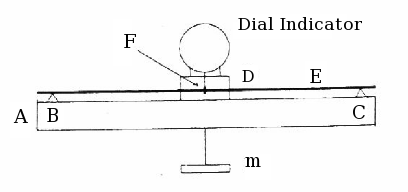
\includegraphics[width=9cm]{scripts/figs/aparatus1.png}
      \caption{Apparatus for measuring the deflection of a rod}
      \label{fig:aparatus1}
    \end{figure}

    \begin{figure}[h!]
      \center
      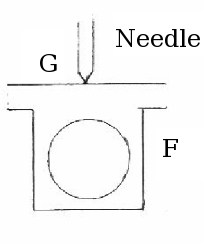
\includegraphics[width=4cm]{scripts/figs/aparatus1cs.png}
      \caption{Cross-section of apparatus where the dial indicator meets the ring in Fig. \ref{fig:aparatus1}}
      \label{fig:aparatus1cs}
    \end{figure}

    The brass rod was placed in an apparatus similar to that which is depicted in Fig. \ref{fig:aparatus1}.  
    
  \subsection{Measuring the speed of sound in the rod}
      The brass rod, with a ring attached to it (same as before), was laid to rest on the flat side of the ring on a solid surface such that the rod is held up by the ring. We also made sure that the rod was not to be disturbed in any way while it was vibrating. When hit with a hammer, it will emit a sound consisting of different frequencies. Following are the two different methods we used for determining the root frequency of the rod.
      During both experiments, we ensured there were no significant noise pollution during our recording (By which i mean people performing the same experiment as us).
      \subsubsection{By hearing for beats}
        A speaker was connected to a signal generator. We started the signal generator at 1200Hz and hit the brass rod with a plastic hammer on the the flat surface on one end of the rod. By ear, there was an audible beat. We adjusted the signal generator such that the the frequency of the beat was minimized, and there was essentially no audible difference between the two signals. We did this by trying above and below where we thought the root frequency was, eventually zeroing in on a value.

      \subsubsection{By Fourier transform}
        A USB microphone was placed close to the rod, and faced towards it. The microphone was connected to a computer running matlab, with a script that collects audio data from it and Fourier transforms it using FFT. The recordings made were made with a sampling frequency of $8\times1024$ Hz and varying durations.



\section{\label{sect:results}Results}

\section{\label{sect:discussion}Discussion}
 
\section{\label{sect:conclusion}Conclusion}

%%%%%%%%%%%%%%%%%%%%%%%%
%%% END OF MAIN BODY %%%
%%%%%%%%%%%%%%%%%%%%%%%%

\bibliography{rapport3_ref}


\onecolumngrid % Start single collumn
\newpage % Ensure Code starts on new page
\section*{Code}
All of the code used to produce this report. Anything noteworthy should already be mentioned in the main body of the report.
\lstinputlisting[language=python]{scripts/lab_data.py}
\lstinputlisting[language=python]{scripts/FYS2150lib.py}

\twocolumngrid % Stop single collumn

\end{document}
